\section{Interferenz}

\subsection{Einleitung}
Bei diesem Experiment soll die Wellenlänge $\lambda$ eines roten und eines grünen Laserpointers bestimmt werden.
Für die Bestimmung wird der Wellencharakter von Licht ausgenutzt, Licht wird nämlich, wenn es auf einen Doppelspalt trifft gebeugt und es entsteht ein Interferenzmuster(Abbildung 1).\\
Zum erzeugen so eines Interferenzmuster wird auf einer optischen Schiene zuerst der Laserpointer befestigt. Dann wird der Doppelspalt so montiert, dass der Lichtstrahl genau darauf trifft,
ans Ende wird dann noch eine Schirm aufgestellt, auf welchem das Interferenzmuster abgebildet wird. Der Abstand zwischen Schirm und Doppelspalt beträgt $d$, diese Größe ist später
zur berechnung der Wellenlänge wichtig. \\
Auf dem Schirm sind die Interferenzmaxima -und minima zu erkennen(Abbildung 1). Zur Berechnung der Wellenlänge braucht man jetzt noch den Abstand $x$ einer bestimmten Zahl an solchen Maxima und die Anzahl
der Maxima über die gemessen wird, wobei man mit 0 anfängt zu zählen.
\begin{figure}[H]
	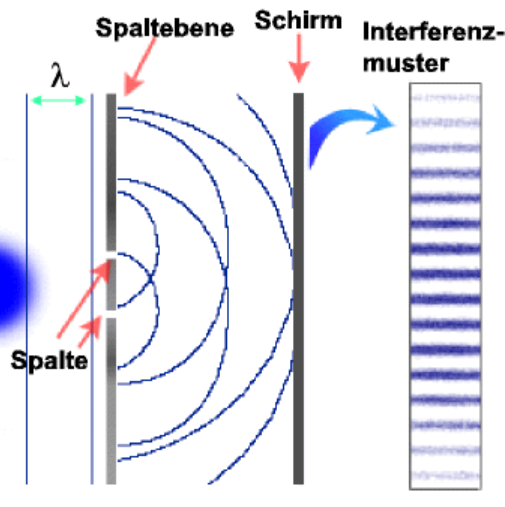
\includegraphics[scale=0.5]{C:/Users/josefk/Desktop/Spektroskopie/src/img/interfernez.PNG}
	\caption{Interferenzmuster welches von Licht erzeugt wird, wenn es auf einen Doppelspalt trifft.}
\end{figure}

\subsection{Berechnung}
\begin{itemize}
	\item Zur bestimmung von $\lambda$ werden zwei Formeln benötigt:
	      \begin{align}
		      \tan \alpha = \frac{x} {d}
	      \end{align}
	      \begin{tabular}{ll}
		      x... Abstand zwischen gemessenen Maxima & d... Abstand vom Schirm zum Doppelspalt \\
		      $\alpha$... Winkel                      &
	      \end{tabular}
	      \begin{align}
		      \sin \alpha = \frac{k\lambda}{a}
	      \end{align}
	      \begin{tabular}{ll}
		      k...Periodizitätfaktor  & a...Spaltabstand des Doppelspalts \\
		      $\lambda$...Wellenlänge &
	      \end{tabular}
	\item Indem man Formel (1) und (2) miteinander Kombiniert, erhält man $\lambda$
	      \begin{align*}
		      \lambda = \frac{a}{k}\sin (\tan^{-1} (\frac{x}{d}))
	      \end{align*}
\end{itemize}
\subsection{Roter Laser}
\begin{table}[H]
	\centering
	\begin{tabular}{lccccc}
		\toprule
		Messung & a [mm] & x [cm] & d [cm] & k [cm] & $\lambda$ [nm] \\
		\midrule
		A1      & 0,3    & 0,9    & 50,7   & 8      & 665,5756152    \\
		A2      & 0,3    & 0,9    & 50,6   & 8      & 666,8905664    \\
		A3      & 0,3    & 1      & 50,6   & 8      & 740,9620347    \\
		A4      & 0,3    & 0,89   & 50,8   & 8      & 656,8873844    \\
		A5      & 0,3    & 0,95   & 50,7   & 8      & 702,5394018    \\
		A6      & 0,3    & 0,978  & 50,7   & 8      & 723,2382344    \\
		\bottomrule
	\end{tabular}
	\caption{Messwerte und daraus resultierende Wellenlänge für den roten Laserpointer}
\end{table}

Die Wellenlänge $\lambda$ des roten Lasers wurde experimentell mit 692,7 $\pm$ ...nm bestimmt.

\subsection{Grüner Laser}

Der Aufbau und Durchführung sind genauso wie beim vorherigen Versuch durchgeführt worden, es wurde einzig der rote Laser mit einem grünen getauscht.

\begin{table}[H]
	\centering
	\begin{tabular}{lccccc}
		\toprule
		Messung & a [mm] & x [cm] & d [cm] & k [cm] & $\lambda$ [nm] \\
		\midrule
		B1      & 0,3    & 0,89   & 50,7   & 10     & 526,5460972    \\
		B2      & 0,3    & 0,9    & 50,6   & 10     & 533,5124531    \\
		B3      & 0,3    & 0,91   & 50,6   & 10     & 539,4384632    \\
		B4      & 0,3    & 0,9    & 50,8   & 10     & 531,4126708    \\
		B5      & 0,3    & 0,92   & 50,7   & 10     & 544,289095     \\
		B6      & 0,3    & 0,92   & 50,7   & 10     & 544,289095     \\
		\bottomrule
	\end{tabular}
	\caption{Messwerte und daraus resultierende Wellenlänge für den roten Laserpointer}
\end{table}

Die Wellenlänge $\lambda$ des grünen Lasers wurde experimentell mit 536,6 $\pm$ ...nm bestimmt.

\subsection{Diskussion}
Wie man in Abbildung 2 sehr gut erkennen kann, passen die experimentell ermittelten Wellenlängen sehr gut mit den theoretischen überein.
Der rote Laserpointer sollte eine Wellenlänge zwischen 640 bis 700 nm und der grüne zwischen 500 und 540 nm haben.\\
Der problematischst Teil war die Messung des Abstandes $x$ zwischen den Maxima, da die grenzen nicht klar und scharf waren, sondern eher verschwommen. Dies Tatsache wird dann später in die 
Fehlerrechnung mit eingehen.   
\begin{figure}[H]
    \centering
	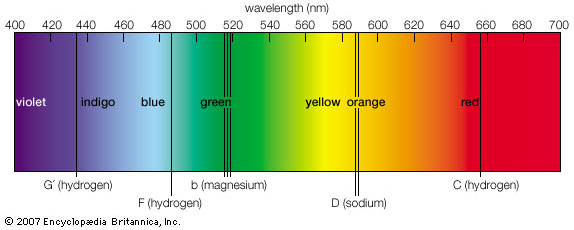
\includegraphics[scale=0.5]{C:/Users/josefk/Desktop/Spektroskopie/src/img/spektrum.PNG}
	\caption{Wellenlängen des sichtbaren Lichts}
\end{figure}
